%% This is file 'chapter1.tex'
%% It is included by hhuthesis-example.tex for hhuthesis.
%%
%% Copyright(C) 2020-2021, Wenhan Cao
%% College of Water Conservancy and Hydropower Engineering, Hohai University.
%%
%% Version:v2.0.0
%% Last update: April 7th, 2021.
%%
%% Home Page of the Project: https://github.com/caowenhan/thesis
%%
%% This file may be distributed and / or modified under the conditions of the
%% LaTeX Project Public License, either version 1.3c of this license or (at your
%% option) any later version. The latest version of this license is in:
%%
%% http://www.latex-project.org/lppl.txt
%%
%% and version 1.3c or later is part of all distributions of LaTeX version
%% 2008/05/04 or later.
%%
\chapter{绪论}
\label{chap:introduction}
\section{河网水力及水质特性数值模拟研究的意义}
\label{sec:meaning}

随着近年来工农业生产的迅猛发展,在河网地区,水资源的供给与需求、环境质量与经济发展这两对矛盾日益突出\cite{tongjiju1997}。环境质量的日趋恶化将愈来愈威胁着区域经济的健康发展,环境治理已成为亟待解决的重大课题\cite{zhengxiaoyu1994}。……\par
……\par
……\par

\section{河网水力及水质特性数值模拟研究综述}

\subsection{水力模拟研究综述}
河网非恒定流的水力特性模拟研究时水利、航运及环保等部门经常进行的工作\cite{liyitian1997}。由于河网区域范围广大,因此只能采用数值方法进行模拟。……\par
……\par
……

\subsubsection{水力数值模拟方法研究}
按控制方程及对河网处理方式的不同,数值模拟方法可分为两大类:第一类为人们所熟知的圣维南方程组求解法,第二类为由法国Jean A.Cunge提出的所谓“组合单元法”\cite{halts1996}。……\par
……\par
……\par
……

\section{技术路线和研究内容}
作为本文核心部分,作者深入系统地研究了平原河网水量水质数值模拟的正反两方面的问题。首次提出用“组合单元法”数值模拟平原河网水力水质特性,分别给出了水量、水质数值模拟的正问题的稀疏矩阵求解方程式及单元分组求解方程式,为平原河网水量水质数值计算开辟了一条新的途径。在正问题的基础上,首次提出:生成基本解,用基本解构造水质边界条件反问题及源项反问题,并采用优化方法中诸如简约梯度法等方法以及遗传算法等方法分别对无约束及有约束的非线性规划问题进行求解。……\par
……\par
……\par
本文的主要研究内容见图\ref{fig:maincontents}。

\begin{figure}[H]
	\centering
	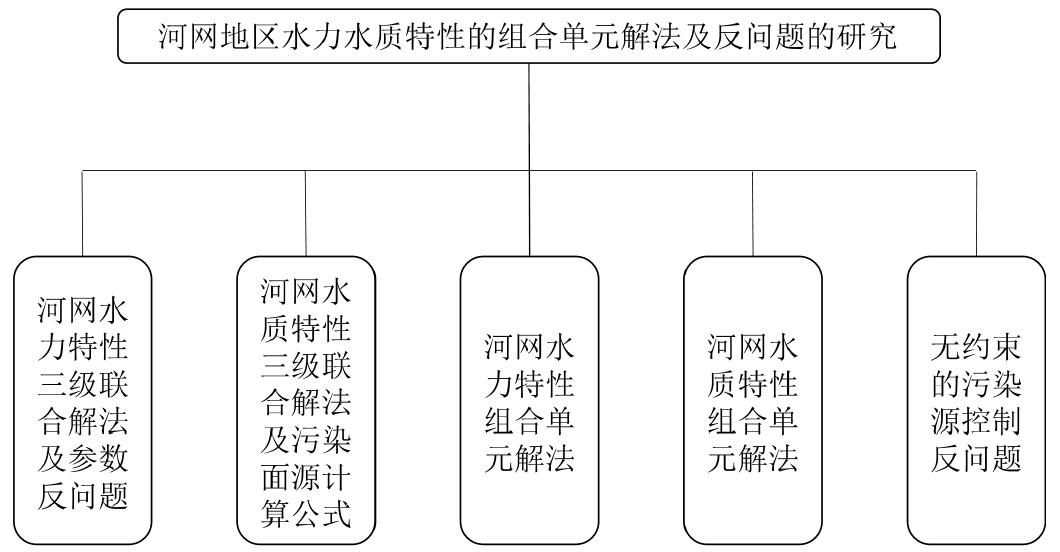
\includegraphics[width=0.75\textwidth]{figure1.jpg}
	\bicaption{论文的主要研究内容}{Main contents of the dissertation}\label{fig:maincontents}
	%硕士论文、本科毕业论文不使用双语图表标题,可使用命令\caption{}替代\caption{}
\end{figure}

